\documentclass{report}
\usepackage[utf8]{vietnam}
\usepackage[utf8]{inputenc}
\usepackage{graphicx}
\usepackage[vietnamese]{babel}
\usepackage[T1]{fontenc}
\usepackage{fouriernc} 
\usepackage{multicol}
\usepackage{listings}
\usepackage{color}
\usepackage{tikz}
\usepackage[most]{tcolorbox}

\newtcbtheorem{theo}%
    {Theorem}{}{theorem}

\definecolor{dkgreen}{rgb}{0,0.6,0}
\definecolor{gray}{rgb}{0.5,0.5,0.5}
\definecolor{mauve}{rgb}{0.58,0,0.82}


\definecolor{codegreen}{rgb}{0,0.6,0}
\definecolor{codegray}{rgb}{0.5,0.5,0.5}
\definecolor{codepurple}{rgb}{0.58,0,0.82}
\definecolor{backcolour}{rgb}{0.95,0.95,0.92}

\lstdefinestyle{mystyle}{
    backgroundcolor=\color{backcolour},   
    commentstyle=\color{codegreen},
    keywordstyle=\color{magenta},
    numberstyle=\tiny\color{codegray},
    stringstyle=\color{codepurple},
    basicstyle=\ttfamily\footnotesize,
    breakatwhitespace=false,         
    breaklines=true,                 
    captionpos=b,                    
    keepspaces=true,                 
    numbers=left,                    
    numbersep=5pt,                  
    showspaces=false,                
    showstringspaces=false,
    showtabs=false,                  
    tabsize=2
}

\lstset{style=mystyle}

\setlength{\parskip}{0.5\baselineskip}
\usepackage[colorlinks=true, urlcolor=blue, linkcolor=red]{hyperref}


\begin{document} 

\begin{titlepage}

	\centering % Centre everything on the title page
	\scshape % Use small caps for all text on the title page
	\vspace*{\baselineskip} 
	\rule{\textwidth}{1.6pt}\vspace*{-\baselineskip}\vspace*{2pt} % Thick horizontal rule
	\rule{\textwidth}{0.4pt} % Thin horizontal rule
	
	\vspace{0.75\baselineskip} 
	
	{\LARGE Chương trình minh họa thuật toán\\ First Come First Serve và\\ Elevator Algorithm\\} % Title
	
	\vspace{0.75\baselineskip} % Whitespace below the title
	
	\rule{\textwidth}{0.4pt}\vspace*{-\baselineskip}\vspace{3.2pt} % Thin horizontal rule
	\rule{\textwidth}{1.6pt} % Thick horizontal rule
	
	\vspace{2\baselineskip} 
	
		Operating Systems(OSG202) % Subtitle or further description
	
	\vspace*{3\baselineskip} % Whitespace under the subtitle
	Edited By
	
	\vspace{0.5\baselineskip} % Whitespace before the editors
	
	{\scshape\Large Nguyễn Thiện Phúc [He186083] \\ Nguyễn Đức Thắng [HE186090] \\} % Editor list
	
	\vspace{0.5\baselineskip} % Whitespace below the editor list
	
	\textit{FPT University\\ Hoa Lac, Ha Noi, Viet Nam} % Editor affiliation
         \begin{center}
             
\includegraphics[width = 5cm]{images/FPTUCT.png}
         \end{center}
	\vfill 
	\vspace{0.3\baselineskip}
	
	July, 2023 % Publication year
	

\end{titlepage}

\tableofcontents{}

\chapter{Giới thiệu}
    \section{Giới thiệu về nhóm}

    Nhóm chúng tôi gồm có 2 sinh viên đều thuộc chuyên ngành Software Engineer là Nguyễn Thiện Phúc và Nguyễn Đức Thắng. Nhóm được lập ra trên cơ sở hợp tác để minh họa lại 2 thuật toán FIRST COME FIRST SERVE và ELEVATOR nhằm phục vụ cho môn học OSG202 ( Operations System ) được chỉ dạy bởi thầy Ngô Hải Anh.
    
    Báo cáo này tóm tắt những nội dung về phần thuyết trình trong môn học OSG202. OSG20 là một môn học được học trong học kỳ 2 của chuyên ngành SE. Trong báo cáo này, chúng e, trình bày các khái niệm, trình bày 2 thuật toán và phần chương trình.

    \section{Giới thiệu về thuật toán}
    \subsection{Disk Scheduling Algorithm}

    \textbf{Disk Scheduling} được thực hiện bởi hệ điều hành để lên lịch các yêu cầu I/O đến đĩa. \textbf{Disk Scheduling} còn được gọi là \textbf{I/O Scheduling}. Disk Scheduling rất quan trọng vì:

    \begin{itemize}
        \item Nhiều yêu cầu I/O có thể đến bởi các quy trình khác nhau và chỉ một yêu cầu I/O có thể được bộ điều khiển đĩa phục vụ tại một thời điểm. Do đó, các yêu cầu I/O khác cần đợi trong hàng đợi và cần được lên lịch.
        
        \item Hai hoặc nhiều yêu cầu có thể cách xa nhau, do đó có thể dẫn đến chuyển động của nhánh đĩa lớn hơn. 
        
        \item Ổ đĩa cứng là một trong những phần chậm nhất của hệ thống máy tính và do đó cần phải được truy cập một cách hiệu quả.
    \end{itemize} 
    
    Có nhiều thuật toán lập lịch đĩa nhưng trước khi thảo luận về chúng, chúng ta hãy xem nhanh một số thuật ngữ quan trọng:

    \textbf{Seek Time} (Thời gian tìm kiếm) : Thời gian tìm kiếm là thời gian cần thiết để xác định vị trí của nhánh đĩa đến một rãnh cụ thể nơi dữ liệu sẽ được đọc hoặc ghi. Vì vậy, thuật toán lập lịch đĩa cung cấp thời gian tìm kiếm trung bình tối thiểu sẽ tốt hơn.
    
    \textbf{Rotation Latency} (Độ trễ quay): Độ trễ quay là thời gian mà khu vực mong muốn của đĩa cần để xoay vào một vị trí sao cho nó có thể truy cập vào các đầu đọc/ghi. Vì vậy, thuật toán lập lịch đĩa cung cấp độ trễ quay tối thiểu sẽ tốt hơn.
    
    \textbf{Transfer Time} (Thời gian truyền): Thời gian truyền là thời gian truyền dữ liệu. Nó phụ thuộc vào tốc độ quay của đĩa và số byte được truyền.
    
    \textbf{Disk Access Time} (Thời gian truy cập đĩa): Thời gian truy cập đĩa là:

    \begin{tcolorbox}
    
    \begin{tabbing}
    Disk Access Time =  \= Seek Time + \\
                        \> Rotational Latency + \\
                        \> Transfer Time \\
    \end{tabbing}
    
      Total Seek Time = Total head Movement * Seek Time
    \end{tcolorbox} 

    \textbf{Disk Response Time} (Thời gian phản hồi của đĩa): Thời gian phản hồi là thời gian trung bình mà một yêu cầu sử dụng để chờ thực hiện thao tác I/O của nó. Thời gian phản hồi trung bình là thời gian phản hồi của tất cả các yêu cầu. Thời gian phản hồi phương sai là thước đo cách yêu cầu riêng lẻ được phục vụ đối với thời gian phản hồi trung bình. Vì vậy, thuật toán lập lịch đĩa cung cấp thời gian phản hồi phương sai tối thiểu sẽ tốt hơn.

    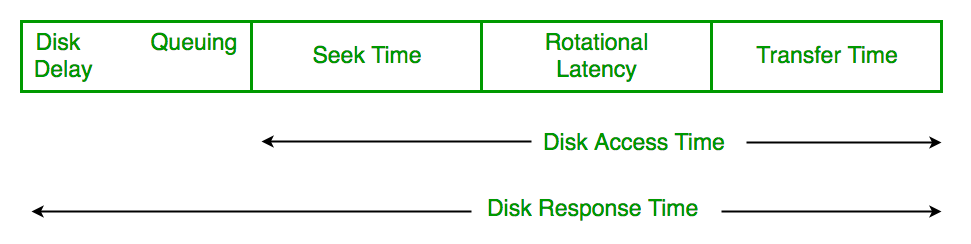
\includegraphics[width = 12cm]{images/disc-scheduling-algorithms.png}

    Được tham khảo từ: \href{https://www.geeksforgeeks.org/disk-scheduling-algorithms/}{https://www.geeksforgeeks.org/disk-scheduling-algorithms/}
        
    \subsection{First Come First Serve (FCFS) Algorithm}

    \textbf{FCFS} là viết tắt của \textbf{First Come First Serve}. Trong thuật toán FCFS, công việc đến đầu tiên trong hàng đợi sẵn sàng được phân bổ cho CPU và sau đó là công việc đến thứ hai, v.v. Có thể nói rằng hàng đợi sẵn sàng hoạt động như một hàng đợi \textbf{FIFO} (Vào trước ra trước), do đó các công việc/quy trình đến được đặt ở cuối hàng đợi.  

    \textbf{FCFS} là một thuật toán lập lịch không ưu tiên vì một quá trình giữ CPU cho đến khi nó kết thúc hoặc thực hiện I/O. Như vậy, nếu một công việc dài hơn đã được gán cho CPU thì nhiều công việc ngắn hơn sau nó sẽ phải đợi. Thuật toán này được sử dụng trong hầu hết các batch operating system. 

    \textbf{FCFS} là thuật toán \textbf{Disk Scheduling} đơn giản nhất. Như tên gợi ý, thuật toán này xử lý các yêu cầu theo thứ tự chúng đến trong hàng đợi đĩa. Thuật toán trông rất công bằng và không có tình trạng chết (tất cả các yêu cầu đều được phục vụ tuần tự) nhưng nhìn chung, nó không cung cấp dịch vụ nhanh nhất.

    \textbf{Thuật toán}: 
    \begin{enumerate}
        \item 
            Đặt mảng \textbf{Request} là một mảng lưu trữ giá trị của tracks đã được yêu cầu theo thứ tự tăng dần về thời gian đến của chúng. '\textbf{head}' là vị trí của đầu đĩa.
    
        \item 
            Chúng ta hãy lần lượt theo dõi các \textbf{tracks} theo thứ tự mặc định và tính khoảng cách tuyệt đối của \textbf{tracks} từ \textbf{head}.
        \item 
            Tăng tổng số lần tìm kiếm với khoảng cách này.
        \item 
            Vị trí \textbf{track} hiện tại trở thành vị trí \textbf{head} mới.
        \item 
            Quay lại bước 2 cho đến khi tất cả các \textbf{tracks} trong mảng \textbf{Requests} được thực thi hết.
    \end{enumerate}

    Ví dụ:

    \begin{tcolorbox}
    
        Input: 
        
        Request sequence = {176, 79, 34, 60, 92, 11, 41, 114}
        
        Initial head position = 50\\
        
        Output:
        
        Total number of seek operations = 510
        
        Seek Sequence is 176 79 34 60 92 11 41 114
        
    \end{tcolorbox} 

    Biểu đồ sau đây cho thấy trình tự các \textbf{requested tracks} được tính bằng FCFS. 

    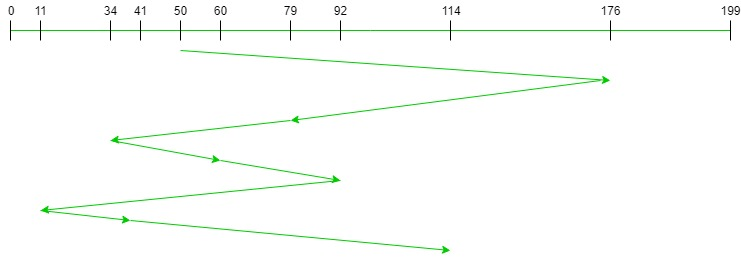
\includegraphics[width = 12cm]{images/fcfs/fcfs-1.jpg}

    Được tham khảo từ: \href{https://www.geeksforgeeks.org/fcfs-scheduling-full-form/}{https://www.geeksforgeeks.org/fcfs-scheduling-full-form/},
    \href{https://www.geeksforgeeks.org/fcfs-disk-scheduling-algorithms/}{https://www.geeksforgeeks.org/fcfs-disk-scheduling-algorithms/}
        
    \subsection{Elevator Algorithm}

    \textbf{Thuật toán Elevator (Scan):}
    
    Trong thuật toán \textbf{Elevator Disk Scheduling}, đầu bắt đầu từ một đầu của disk và di chuyển về phía đầu kia, thực hiện các yêu cầu ở giữa từng cái một và đến đầu kia. Sau đó, hướng của \textbf{head} được đảo ngược và quá trình tiếp tục khi \textbf{head} liên tục quét qua lại để truy cập disk. Vì vậy, thuật toán này hoạt động như một thang máy và do đó được gọi là \textbf{Elevator Algoithm}. Do đó, các yêu cầu ở dải trung được phục vụ nhiều hơn và những yêu cầu đến sau nhánh đĩa sẽ phải đợi.

    \textbf{Thuật toán:} 

    \begin{enumerate}
        \item 
            Đặt mảng \textbf{Request} là một mảng lưu trữ giá trị của các tracks đã được yêu cầu theo thứ tự tăng dần về thời gian đến của chúng. '\textbf{head}' là vị trí của đầu đĩa.
        \item 
            Đặt \textbf{direction} đại diện cho việc \textbf{head} đang di chuyển về phía trái hay phải.
        \item 
            Theo hướng mà \textbf{head} đang di chuyển, tính từng \textbf{track} một.
        \item 
            Tính khoảng cách tuyệt đối của \textbf{track} từ \textbf{head}.
        \item 
            Tăng tổng số lần tìm kiếm với khoảng cách này.
        \item 
            Vị trí \textbf{track} hiện tại bây giờ trở thành vị trí \textbf{head} mới.
        \item 
            Quay lại bước 3 cho đến khi chúng ta đến một trong các đầu của đĩa.
        \item  
            Nếu chúng ta đến cuối đĩa, hãy đảo ngược hướng và quay lại bước 2 cho đến khi tất cả các \textbf{track} trong mảng \textbf{Request} được thực thi hết.
            
    \end{enumerate}

    Ví dụ:

    \begin{tcolorbox}
    
        Input: 
        
        Request sequence = {176, 79, 34, 60, 92, 11, 41, 114}
        
        Initial head position = 50

        Direction = left (Chúng ta di chuyển từ phải sang trái)\\

        Output:

        Total number of seek operations = 226

        Seek Sequence is 41 34 11 0 60 79 92 114 176
    \end{tcolorbox} 

    Biểu đồ sau đây cho thấy trình tự các \textbf{track} được thực hiện bằng \textbf{Elevator Algorithm}. 

    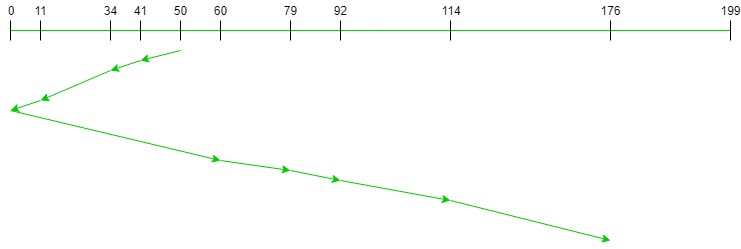
\includegraphics[width = 12cm]{images/elevator/ele-1.jpg}

    Được tham khảo từ: \href{https://www.geeksforgeeks.org/scan-elevator-disk-scheduling-algorithms/}{https://www.geeksforgeeks.org/scan-elevator-disk-scheduling-algorithms/}
    
\chapter{Chương trình}
    \section{Cài đặt và chạy}
        \subsection{Hệ điều hành}
        Chương trình được cài đặt trên hệ điều hành Linux.
        
        Bởi vì hệ điều hành của thầy bọn em không có password của user nên không thể update được g++ compiler. Do đó, chúng em đã cài đặt hệ điều hành \textbf{ArchLinux} để có thể có được môi trường tốt để code và chạy chương trình này

        Bọn em đã cài đặt trên: \href{https://archlinux.org/download/}{ArchLinux Download} và dựa theo clip \href{https://www.youtube.com/watch?v=FlQ-LyBDCoo}{How To Install Arch Linux in VirtualBox (2023) | Arch Linux Installation} để có thể cài đặt \textbf{ArchLinux} một cách ổn nhất có thể.

        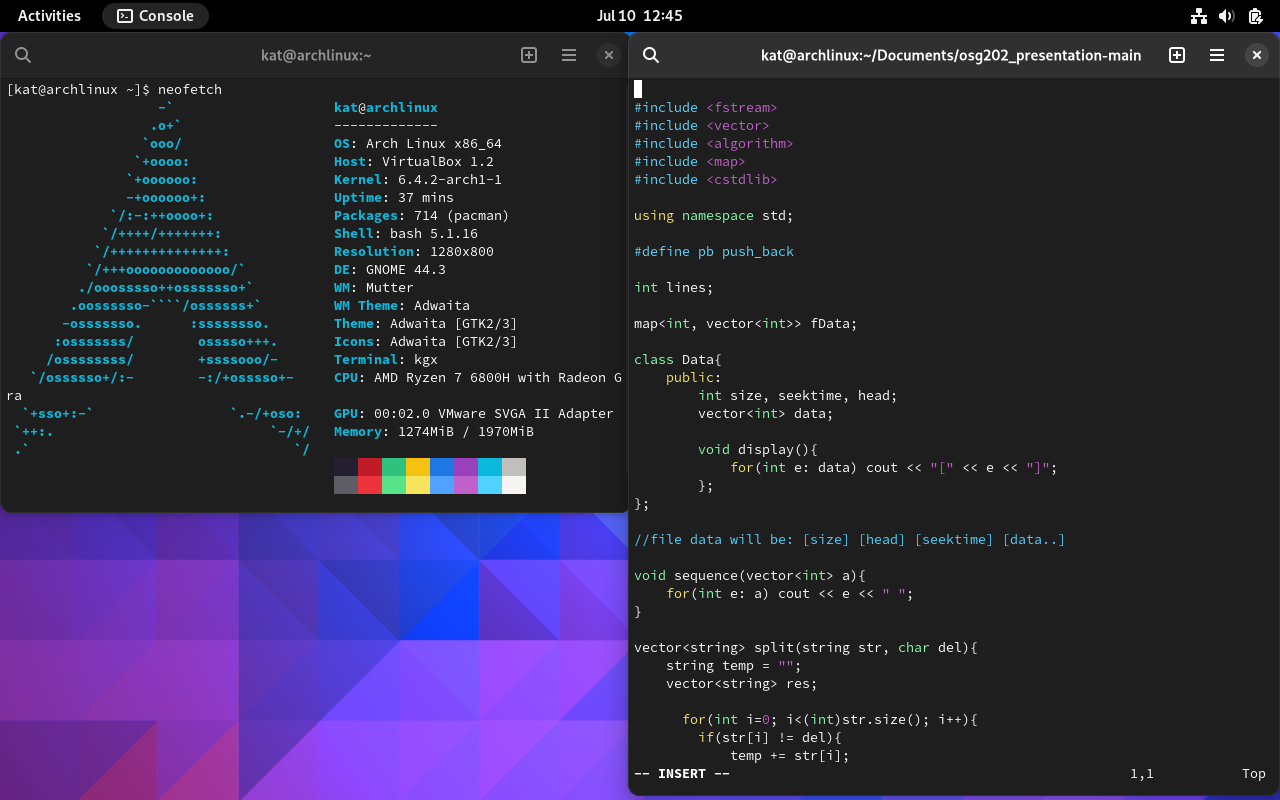
\includegraphics[width = 14cm]{images/archlinux.png}
        
        \subsection{Compiler}
        Chương trình được compile bằng g++ compiler
        Chúng em cài đặt GCC Compiler theo bài viết: \href{https://linuxhint.com/install-gcc-arch-linux/}{How to Install GCC for Arch Linux}.

        G++ Version của bọn em đang sử dụng là: g++ (GCC) 13.1.1

        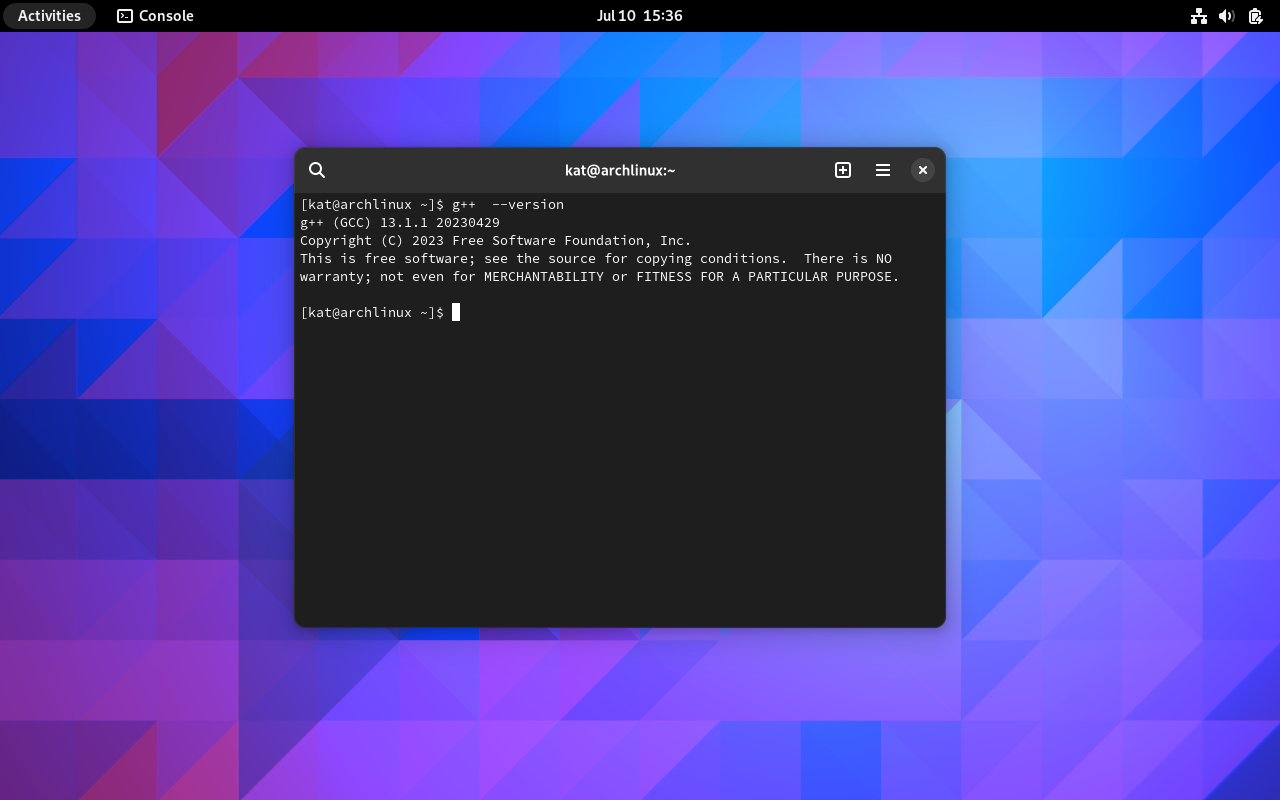
\includegraphics[width = 12cm]{images/g++version.png}
        
        Để code được chương trình thì bọn em còn sử dụng thêm \href{https://www.vim.org/}{Vim} (một ứng dụng biên soạn văn bản). Chương trình này đã được cài đặt sẵn khi cài đặt ArchLinux nên bọn em không cần cài thêm.

        Nếu không có Vim trong máy thì có thể cài đặt theo đường dẫn sau: \href{https://tecadmin.net/install-vim-linux/}{How to Install Latest Vim Editor in Linux}

        \subsection{Cài đặt chương trình}
        Chương trình có thể tải về từ repo: \href{https://github.com/kat1002/osg202_presentation.git}{Chương trình mô phỏng 2 thuật toán FCFS và Elevator}.
        Sau khi tải thì bước tiếp theo là giải nén và chạy file program.
            
    \section{Xử lý dữ liệu}
        Dữ liệu của chương trình sẽ gồm:

        \begin{lstlisting}[language=C++, caption=Data in program]
int lines;

class Data{
    public: 
        int size, seektime, head;
        vector<int> data;
        
        void display(){
            for(int e: data) cout << "[" << e << "]"; 
        };
};
        \end{lstlisting}

        Về phần data:
        \begin{itemize}
            \item \textcolor{red}{lines}: số dòng trong file input.txt
            \item Class Data:
                \begin{multicols}{2}
                    \begin{minipage}{3cm}
                        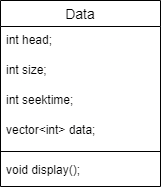
\includegraphics[width=4cm]{images/Data.png}
                    \end{minipage}
                    \hspace{1cm}
                    \begin{minipage}{10cm}
                        \begin{itemize}
                            \item \textcolor{red}{head}: giá trị của cylinder đầu tiên
                            \item \textcolor{red}{size}: số lượng cylinders trong data 
                            \item \textcolor{red}{seektime}: thời gian 1 lần di chuyển cylinder (msec)
                            \item \textcolor{red}{data}: dãy vector<\textcolor{blue}{int}> chứa giá trị của các cylinders
                            \item \textcolor{red}{display()}: Hàm đưa ra console giá trị của tất cả các cylinders trong data
                        \end{itemize}
                    \end{minipage}
                \end{multicols}
        \end{itemize}
        
        Dữ liệu đầu vào và đầu ra sẽ được phân ra làm 2 phần:
        
        \begin{itemize}
            \item Thông qua console
            \item Thông qua file
                
        \end{itemize}
        
        \subsection{Qua console}
            Người dùng sẽ nhập qua console những data cần thiết:
                \begin{itemize}
                    \item head
                    \item size
                    \item seektime
                    \item data
                \end{itemize}

                Dữ liệu đầu ra sẽ được xuất ra console theo format:\\ 
                \begin{tcolorbox}[colback=red!5!white, colframe = red!50!black, title = Console Output]
                    Data: [data[0]] [data[1]] .. [data[n]]\\
                    FCFS seek time: kết quả\\
                    Seek sequence: Thứ tự đọc các cylinders\\
                    Elevator seek time: kết quả\\
                    Seek sequence: Thứ tự đọc các cylinders\\
                \end{tcolorbox}
                
        \subsection{Qua file I/O}
            Người dùng sẽ nhập các input vào trong file "input.txt" và chương trình sẽ chạy dựa theo các input đã được nhập trong "input.txt".

            Các case trong file "input.txt" phải được nhập trên 1 dòng và theo format sau:

            \begin{tcolorbox}[colback=red!5!white, colframe = red!50!black, title = File Input Format]
                    
                [size] [head] [seektime] [data]
            \end{tcolorbox}
            
            Ví dụ:
            \begin{tcolorbox}[colback=gray!5!white,     colframe = gray!50!black, title = input.txt]
                    3 86 17 15 93 35
                    
                    6 92 9 21 62 27 90 59 63
                    
                    6 40 6 72 36 11 68 67 29
                    
                    2 30 2 23 67
            \end{tcolorbox}

            Sau khi lấy được dữ liệu từ "input.txt", chương trình sẽ tự động thực hiện tính toán cả 2 thuật toán FCFS và Elevator.

            Sau khi tính toán xong kết quả sẽ tự động được lưu vào trong file "output.txt" theo format:

            \begin{tcolorbox}[colback=red!5!white, colframe = red!50!black, title = File Output Format]
                    i:\\
                    FCFS: res, Seek sequence: [..]\\
                    Elevator: res, Seek sequence: [..]
            \end{tcolorbox}           

            Ví dụ:
            \begin{tcolorbox}[colback=gray!5!white,     colframe = gray!50!black, title = output.txt]
                    1: \\
                    FCFS: 3519ms, Seek sequence: [15] [93] [35] \\ 
                    Elevator: 3519ms, Seek sequence: [93] [15] [35] \\ 
                    2: \\
                    FCFS: 2205ms, Seek sequence: [21] [62] [27] [90] [59] [63] \\ 
                    Elevator: 2205, Seek sequence: [21] [27] [59] [62] [63] [90] \\
                    3:\\ 
                    FCFS: 1134ms, Seek sequence: [72] [36] [11] [68] [67] [29] \\ 
                    Elevator: 1134, Seek sequence: [67] [68] [72] [11] [29] [36] \\
                    4:\\ 
                    FCFS: 102ms, Seek sequence: [23] [67]\\ 
                    Elevator: 102ms, Seek sequence: [67] [23]\\ 
            \end{tcolorbox}
            
            
            
        
    \section{Chức năng chính}
        Chương trình mô phỏng 2 thuật toán sẽ có các chức năng:
            \begin{itemize}
              \item File Input.
              \item Console Input.
              \item Generate random cases.
              \item Exit
            \end{itemize}
        Người dùng sẽ chọn giữa 4 options bằng cách nhập input từ bàn phím.
        
        \subsection{Console Input}
            
            Option \textbf{Console Input}:
            Người dùng sẽ phải nhập input từ console và chương trình sẽ chạy để tính toán 2 thuật toán và in kết quả ra console.

            \begin{lstlisting}[language=C++, caption=Console Input Function]
void cCase(){
    Data uData;
    vector<int> seek_sequence;
    int fcfs, elevator;

    userInput(uData);
    
    cout << "\nData: "; uData.display();
    fcfs = FCFS(uData.head, uData, seek_sequence);
    cout << "FCFS seek time: " << fcfs << endl;
    cout << "Seek sequence: "; sequence(seek_sequence);
    cout << endl;
    seek_sequence.clear();

    cout << "\nData: "; uData.display();
    elevator = Elevator(uData.head, uData, seek_sequence);
    cout << "Elevator seek time: " << elevator << endl;
    cout << "Seek sequence: "; sequence(seek_sequence); 
    cout << endl;
    seek_sequence.clear();
}
            \end{lstlisting}

            Để có thể lưu trữ dữ liệu được nhập thì em đã viết function \textbf{User Input}:

            \begin{lstlisting}[language=C++, caption = "User Input from Console"]
void userInput(Data &data){
    cout << "Input\n";

    cout << "Number of cylinders: ";
    cin >> data.size;

    cout << "Disk reading from: ";
    cin >> data.head;

    cout << "Seektime: ";
    cin >> data.seektime;

    cout << " Data: ";
    for(int i = 0; i < data.size; ++i) {
        int tmp;
        cin >> tmp;
        data.data.pb(tmp);
    }
}
            \end{lstlisting}

    Chương trình chạy thực tế: \\
    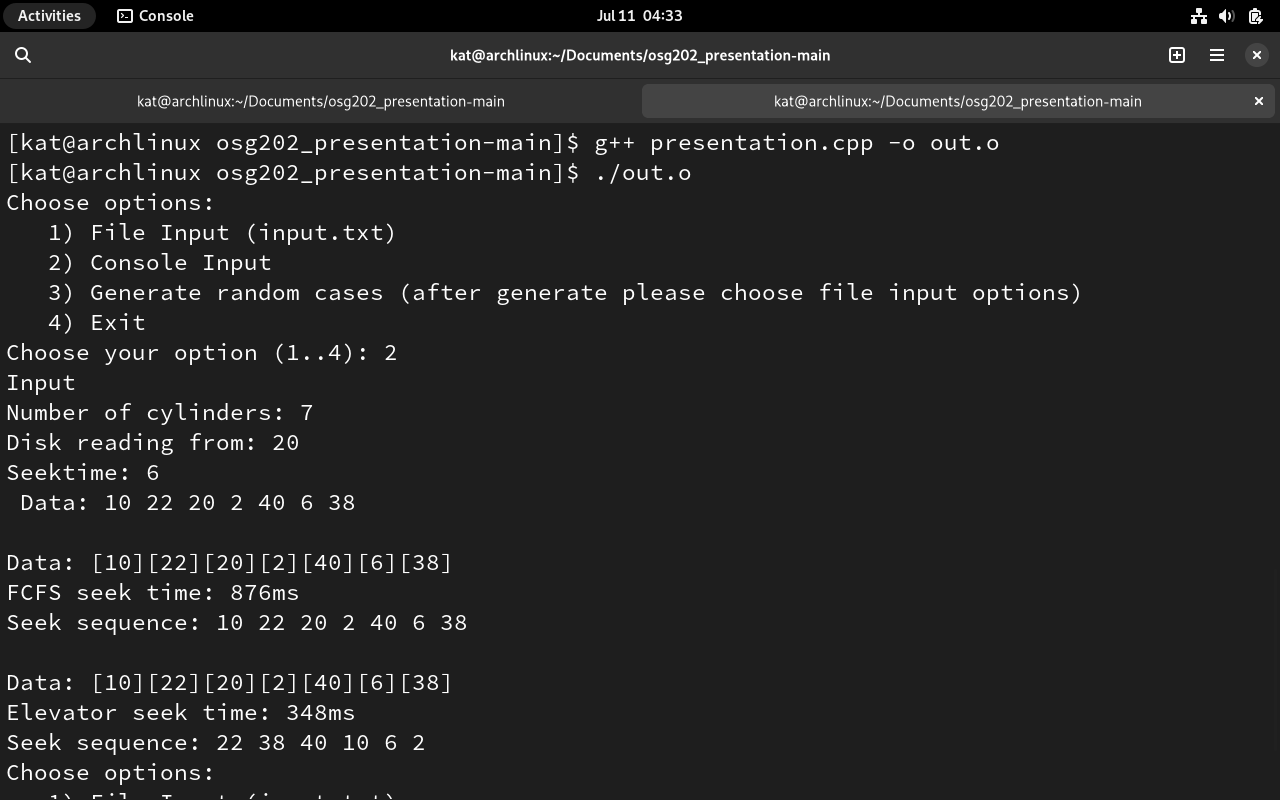
\includegraphics[width = 12cm]{images/consoleinput.png}
            
        \subsection{File Input}
            Option \textbf{File Input}: Người dùng sẽ không cần phải nhập input từ console mà các cases sẽ được tự động nhập từ file "input.txt".
        
            \begin{lstlisting}[language=C++, caption=File Input Function]
void fCase(){
    map<int, Data> fData;
    vector<int> fcfs, elevator;
    vector<vector<int>> fcfs_se, elevator_se;


    fileInput("./input.txt", fData);
    
    for(int i = 0; i < lines; ++i){
        vector<int> fcfs_sequence, elevator_sequence;
        
        fcfs.pb(FCFS(fData[i].head, fData[i], fcfs_sequence));
        elevator.pb(Elevator(fData[i].head, fData[i], elevator_sequence));

        fcfs_se.pb(fcfs_sequence);
        elevator_se.pb(elevator_sequence);
    }

    cout << "All calculations have been done. Please check the output in file \"output.txt\"." << endl;
    
    fileOutput("./output.txt", fcfs, elevator, fcfs_se, elevator_se);
}
            \end{lstlisting}

            Chương trình chạy thực tế: \\
            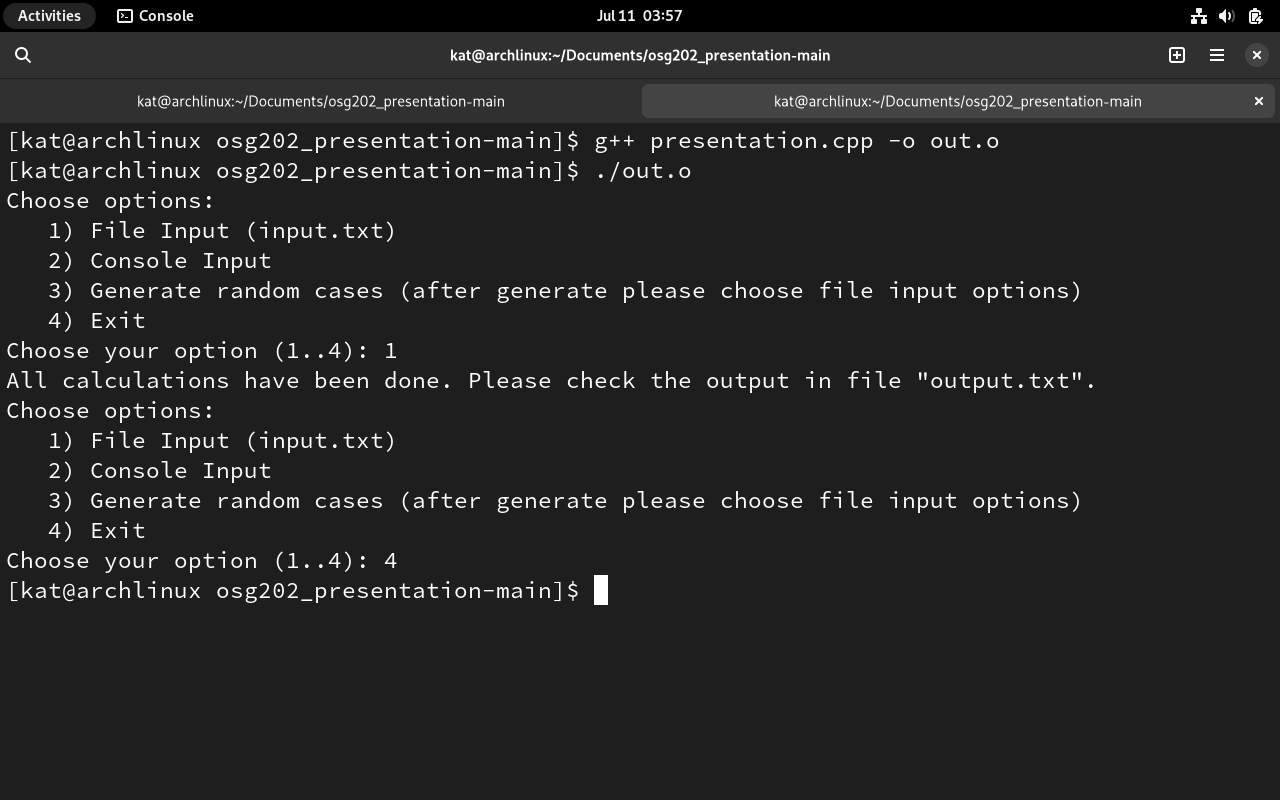
\includegraphics[width = 12cm]{images/fileinput.png}

            File "input.txt":\\
            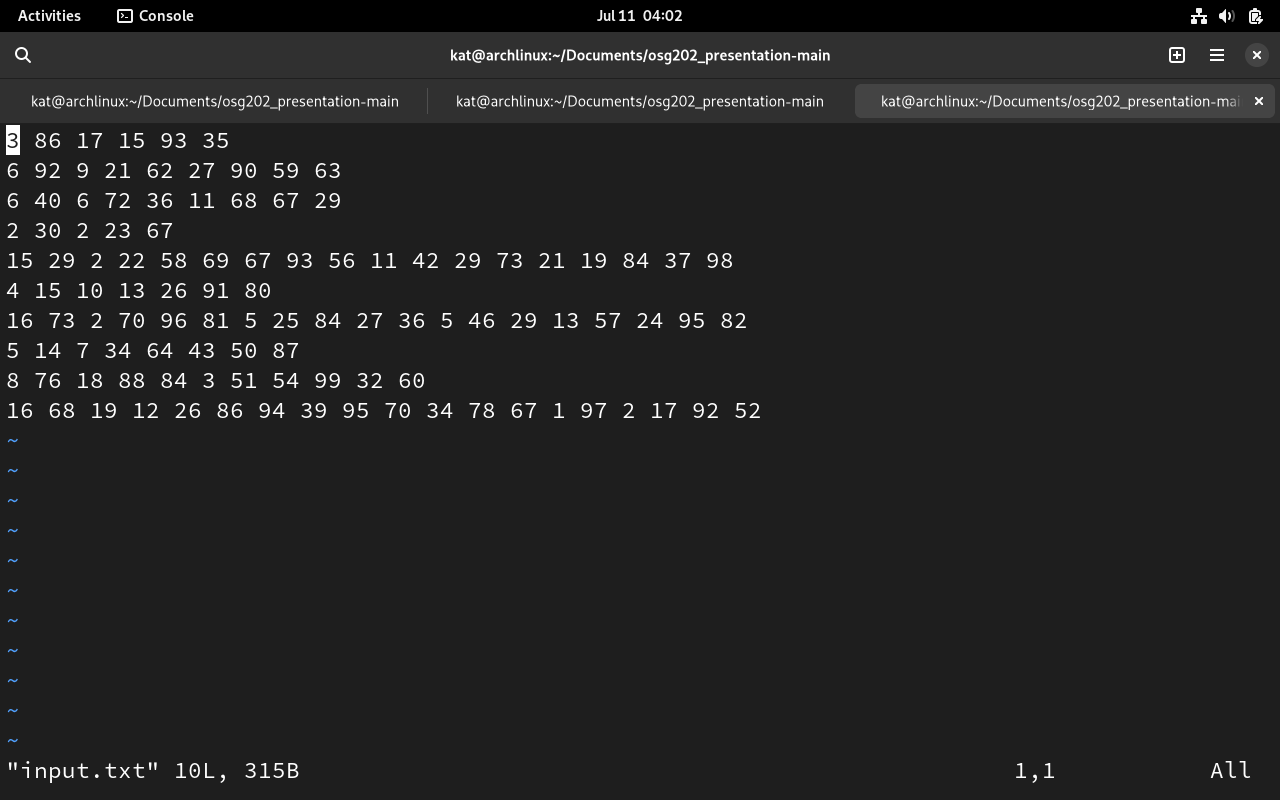
\includegraphics[width=12cm]{images/randominputtxt.png}

            File "output.txt" sau khi chạy function:\\
            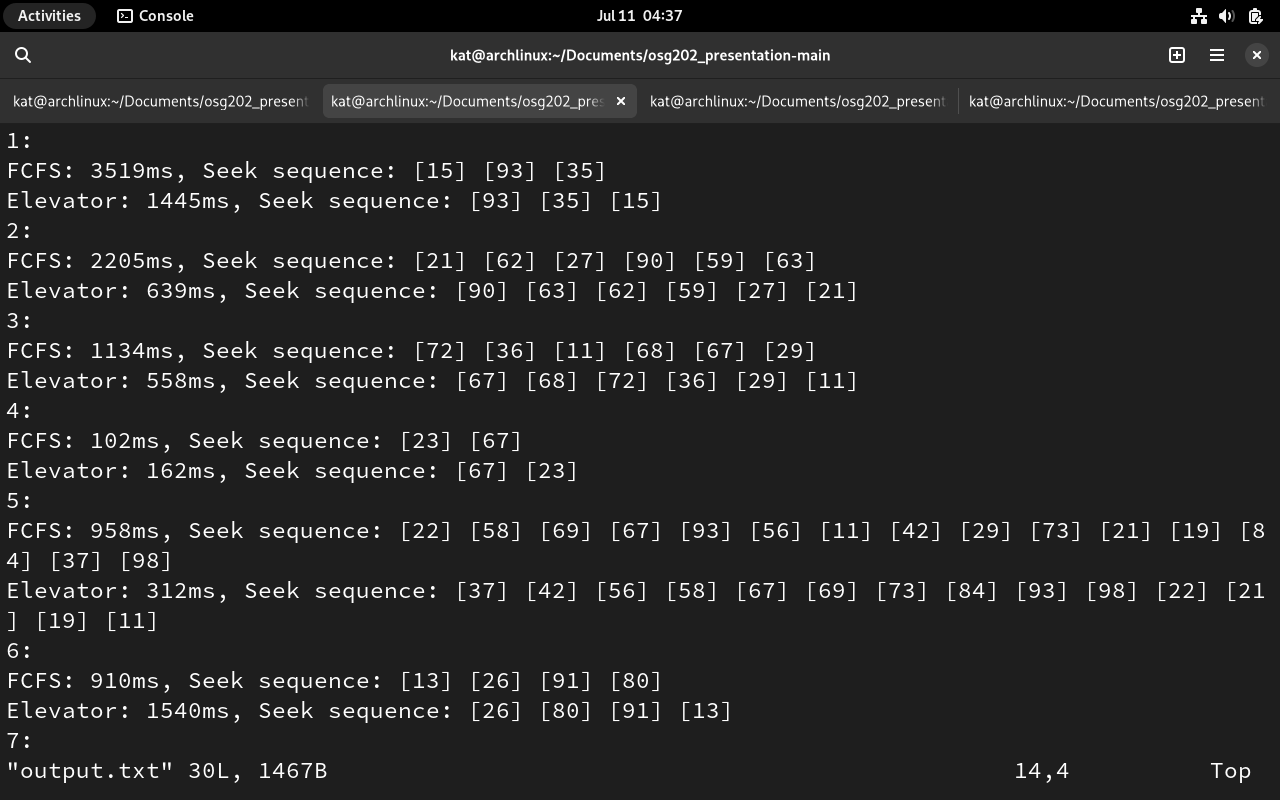
\includegraphics[width=12cm]{images/outputtxt.png}
                        
        \subsection{Generate random cases}
            
            Option \textbf{Generate random cases}:
            Người dùng sẽ phải nhập input từ console và chương trình sẽ chạy để tính toán 2 thuật toán và in kết quả ra console.

            \begin{lstlisting}[language=C++, caption=Generate random cases Function]
void rCase(){
    int N = 100;
    int s = 20;
    int ss = 10;
    int n;
    vector<string> lines;
    cout << "Data random: " << endl;
    cout << "Size: [1..20] | Seektime: [1..10] | Head and data inside: [1..100]" << endl;;
    cout << "Enter numbers of processes: ";
    cin >> n;

    for(int i = 0; i < n; ++i){
        Data rData;
        int tmp;

        random(rData.size, s);
        random(rData.head, N);
        random(rData.seektime, s);	
 
        for(int j = 0; j < rData.size; ++j) rData.data.pb(random(tmp, N));

	string line = to_string(rData.size) + " " + to_string(rData.head) + " " + to_string(rData.seektime);
 
        for(int e : rData.data)
            line += " " + to_string(e);
        line += "\n";
 
        lines.pb(line);
    }

    dataRandomOutput("./input.txt", lines);

    cout << "All random cases have been generated. Please check file \"input.txt\" to have more infomation." << endl;

}
            \end{lstlisting}

            Chương trình chạy thực tế:\\
            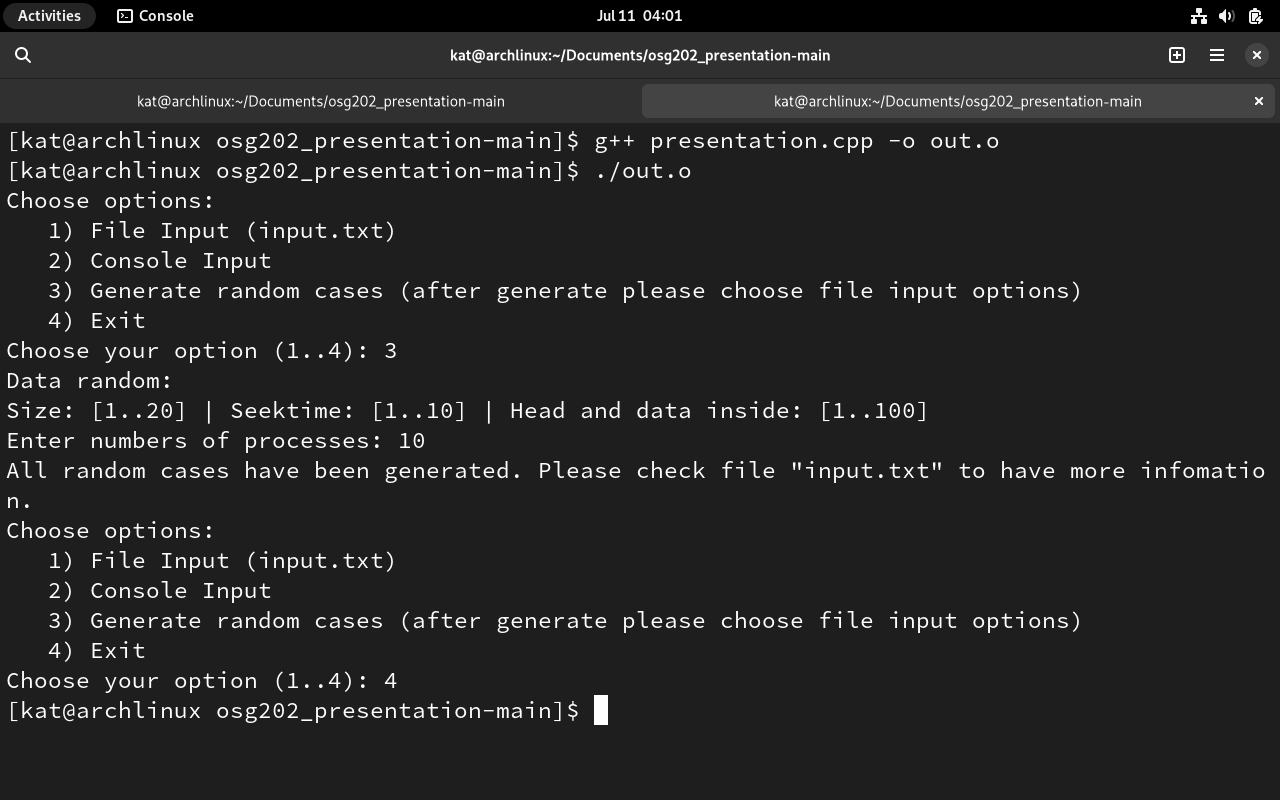
\includegraphics[width = 12cm]{images/randomcases.png}

            File "input.txt" sau khi chạy function:\\
            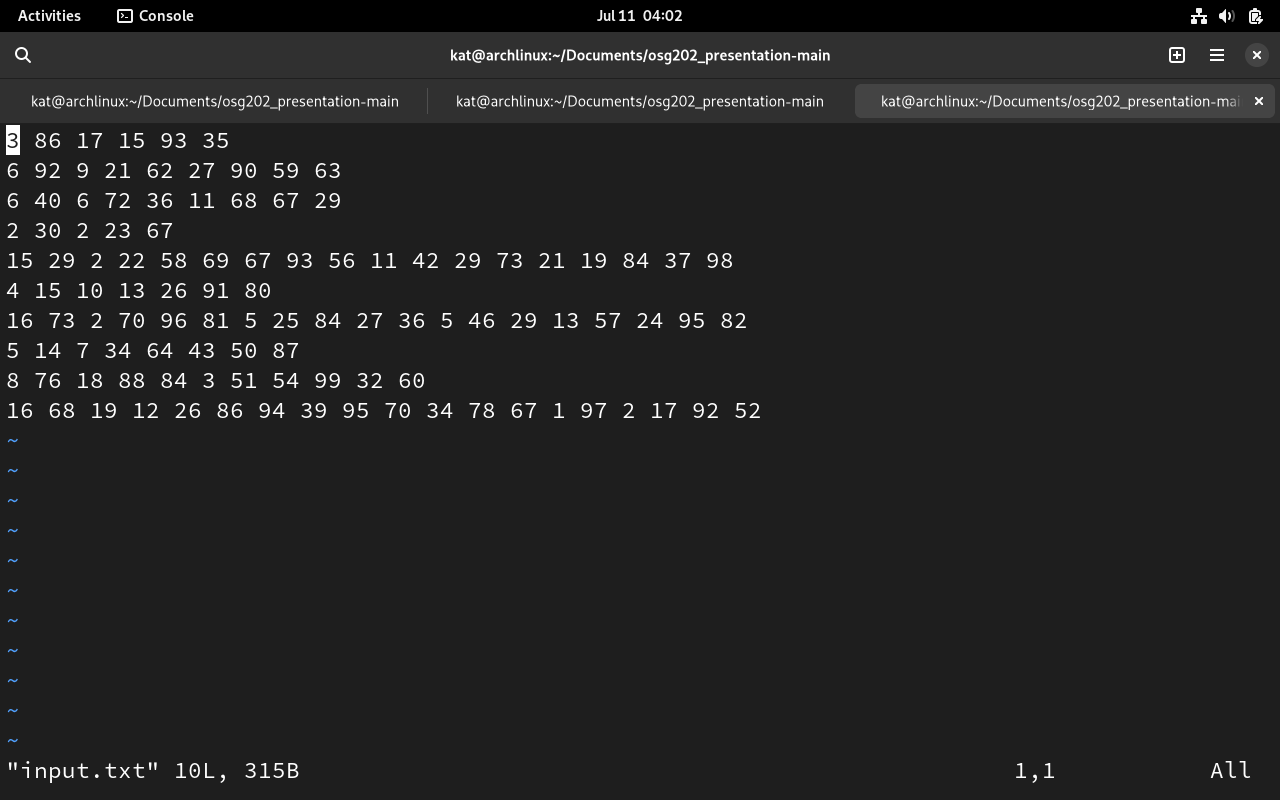
\includegraphics[width = 12cm]{images/randominputtxt.png}

    Để có thể tạo 1 cases random em đã viết thêm 1 funtion \textbf{random()}:

            \begin{lstlisting}[language=C++, caption=Random Function]
int random(int &x, int max){
	x = rand() % max;
	while(x == 0) x = rand() % max;
	return x;
}    
            \end{lstlisting}

            

    \section{Các function}
        Để có thể tính toán và có thể chạy được thì chúng em đã sử dụng các thư viện:

        \begin{lstlisting}[language=C++, caption=Libraries]
#include <iostream>
#include <fstream>
#include <vector>
#include <algorithm>
#include <map>
#include <cstdlib>
#include <string>
        \end{lstlisting}

        Về các function để tính toán những dữ liệu:
        \begin{itemize}
            \item FCFS()
            \item Elevator()
        \end{itemize}

        Trong đó dữ liệu được đưa vào các function:
            \begin{itemize}
                \item \textcolor{red}{head}: giá trị của cylinder đầu tiên
                \item \textcolor{red}{data}: dữ liệu của data được đưa vào (tức case được đưa vào để sử dụng \textbf{FCFS})
                \item \textcolor{red}{seek\_sequence}: thứ tự đọc các cylinders
            \end{itemize}

        
        Và function sẽ trả về dữ liệu tốc độ truy xuất dữ liệu theo kiểu \textcolor{blue}{int}.
            

        \subsection{FCFS}
            Function này dùng để tính toán dữ liệu về thuật toán First Come First Serve.

            \begin{lstlisting}[language=C++,caption=FCFS implementation]
int FCFS(int head, Data data, vector<int>& seek_sequence){
    int res = 0;

    for(int i : data.data){
	seek_sequence.pb(i);
        res += abs(head - i);
        head = i;
    }
    
    return res *= data.seektime;
}
            \end{lstlisting}

        \subsection{Elevator}
            Function này dùng để tính toán dữ liệu về thuật toán Elevator. Ở đây chúng em xin được tính theo chiều từ trái sang phải (\textbf{direction} = left).

            \begin{lstlisting}[language=C++, caption = Elevator Implementation]
int Elevator(int head, Data data, vector<int>& seek_sequence){
    int res = 0;
    int distance;
    vector<int> left, right;


    for(int o : data.data){
        if(o > head) right.pb(o);
        if(o < head) left.pb(o);
    }

    sort(left.begin(), left.end());
    sort(right.begin(), right.end());

    for(int o : right){
        seek_sequence.pb(o);
        res += abs(head - o);
        head = o;
    }

    for(int i = left.size() - 1; i >= 0; i--){
        int o = left[i];
	seek_sequence.pb(o);
        res += abs(head - o);
        head = o;
    }

    return res *= data.seektime;
}

            \end{lstlisting}

        \subsection{Đọc/ghi file}
            Để có thể sử dụng dữ liệu từ file chúng em sử dụng thư viện \textbf{<fstream>}.

            \subsubsection{Đọc file}
                \begin{lstlisting}[language=C++, caption=File Reading]

void fileInput(string path, map<int, Data>& fData){
    ifstream input(path);
    
    string line;
    lines = 0;

    while(!input.eof()){
        Data tmpData;
        vector<string> element;
        
        input >> tmpData.size;
        input >> tmpData.head;
        input >> tmpData.seektime;

        for(int i = 0; i < tmpData.size; ++i){
            int tmp;
            input >> tmp;
            tmpData.data.pb(tmp);
        }
        
        fData.insert(pair<int, Data>(lines, tmpData));
        ++lines;
    }
    lines--;	
    input.close();
}
    
                \end{lstlisting}

                Dữ liệu được nhập vào function:
                \begin{itemize}
                    \item \textcolor{red}{path}: Đường dẫn đến file input
                    \item \textcolor{red}{fData}: Map chứa dữ liệu Data để có thể lưu
                \end{itemize}

            \subsubsection{Ghi file}
                \begin{lstlisting}[language=C++, caption = File writing (Output)]           
void fileOutput(string path, vector<int> fcfs, vector<int> elevator, vector<vector<int>> fcfs_sequence, vector<vector<int>> elevator_sequence){
    
    fstream output;
    output.open(path, std::ofstream::out | std::ofstream::trunc);

    for(int i = 0; i < lines; ++i){
        string line = "";
        line += to_string(i+1) + ": \n";
        line += "FCFS: " + to_string(fcfs[i]) + "ms, Seek sequence: ";
        for(int x : fcfs_sequence[i]) line += "[" + to_string(x) + "] ";
        line += "\n";
        
        line += "Elevator: " + to_string(elevator[i]) + "ms, Seek sequence: ";
        for(int x : elevator_sequence[i]) line += "[" + to_string(x) + "] ";
        output << line << endl;
    }

    output.close();
}
                \end{lstlisting}
                
                Dữ liệu được nhập vào function:
                \begin{itemize}
                    \item \textcolor{red}{path}: Đường dẫn đến file input
                    \item \textcolor{red}{fcfs}: Mảng Vector chứa kết quả từ thuật toán \textbf{FCFS}
                    \item \textcolor{red}{elevator}: Mảng Vector chứa kết quả từ thuật toán \textbf{Elevator}
                    \item \textcolor{red}{fcfs\_sequence}: Mảng Vector chứa các mảng thứ tự đọc cylinders của các cases của thuật toán \textbf{FCFS}
                    \item \textcolor{red}{elevator\_sequence}: Mảng Vector chứa các mảng thứ tự đọc cylinders của các cases của thuật toán \textbf{Elevator}
                \end{itemize}

            \subsubsection{Lưu dữ liệu random vào file}
                \begin{lstlisting}[language=C++, caption = Tạo dữ liệu random]
void dataRandomOutput(string path, vector<string> lines){
    fstream output;
    output.open(path, std::ofstream::out | std::ofstream::trunc);

    for(string line : lines) output<<line;

    output.close();
}
                \end{lstlisting}

                 Dữ liệu được nhập vào function:
                \begin{itemize}
                    \item \textcolor{red}{path}: Đường dẫn đến file input
                    \item \textcolor{red}{lines}: Mảng Vector chứa các dữ liệu input được tạo từ thuật toán random
                    
                \end{itemize}
\chapter{Nhận xét}
    \section{First-Come, First Serve}
        \begin{enumerate}
            \item[-] Hoạt động: FCFS xử lý các yêu cầu I/O theo thứ tự chúng được gửi đến hệ thống. Điều này có nghĩa là yêu cầu nào đến trước sẽ được xử lý trước.

            \item[-] Ưu điểm:
                \begin{enumerate}
                    \item[.] Đơn giản và dễ hiểu.
                    \item[.] Không gây ra độ trễ cho các yêu cầu đến sau.
                \end{enumerate}
            \item[-] Nhược điểm:
                \begin{enumerate}
                    \item[.] Không tối ưu hóa việc di chuyển đầu đọc/ghi đĩa.
                    \item[.] Có thể gây ra hiện tượng "đói" đĩa (starvation) cho các yêu cầu ở vị trí xa.
                \end{enumerate} 
        \end{enumerate}

    \section{Elevator (SCAN)}
        \begin{enumerate}
            \item[-] Hoạt động: Elevator di chuyển đầu đọc/ghi đĩa từ một đầu đến đầu kia, xử lý các yêu cầu I/O trên đường đi và không quay lại trước khi đến đầu đĩa. Nếu không có yêu cầu nào trên đường đi, nó sẽ thay đổi hướng di chuyển và tiếp tục quét theo hướng ngược lại.

            \item[-] Ưu điểm:
                \begin{enumerate}
                    \item[.] Tối ưu hóa việc di chuyển đầu đọc/ghi đĩa bằng cách di chuyển liên tục trong một hướng duy nhất.
                    \item[.] Tránh hiện tượng "đói" đĩa bằng cách xử lý yêu cầu trên đường đi của đầu đọc/ghi đĩa.
                \end{enumerate}
            \item[-] Nhược điểm:
                \begin{enumerate}
                    \item[.] Có thể gây ra độ trễ lớn cho các yêu cầu mới đến nếu chúng không nằm trên đường đi của đầu đọc/ghi đĩa.
                \end{enumerate}
        \end{enumerate}


    \section{So sánh}
        Cả hai thuật toán tìm kiếm Cylinder đều có ưu điểm và nhược điểm khác nhau.\\

        \begin{center}
            
        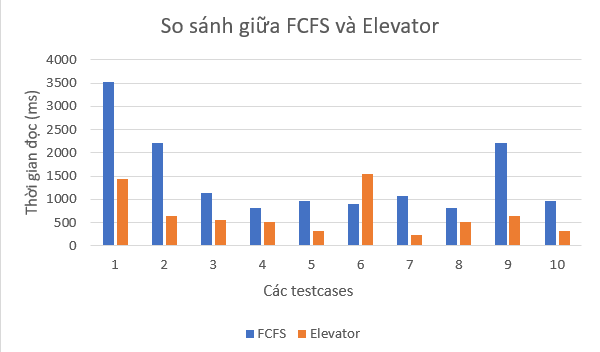
\includegraphics[width=12cm]{images/chartsosanh.png}
        
        ĐỒ THỊ THỂ HIỆN THỜI GIAN GIỮA 2 THUẬT TOÁN TRONG 10 TESTCASES KHÁC NHAU
        \end{center}
        
        \subsection{Độ phức tạp thời gian}
            \begin{itemize}
                \item \textbf{FCFS}: Thuật toán này có độ phức tạp thời gian là O(\(n\)), trong đó n là số lượng yêu cầu tìm kiếm cylinder. Vì thuật toán chỉ đơn giản lựa chọn yêu cầu theo thứ tự đến, nên không có bước tính toán phức tạp.
    
                \item \textbf{Elevator}: Thuật toán Elevator có độ phức tạp thời gian trung bình là O(\(n\)), với n là số lượng yêu cầu tìm kiếm cylinder. Tuy nhiên, trong trường hợp xấu nhất, độ phức tạp có thể là O(\(n^2\)), nếu có yêu cầu tìm kiếm ở cả hai hướng và phải đi qua toàn bộ đĩa.
                
            \end{itemize}
    
    
        \subsection{Hiệu suất tìm kiếm}
            \begin{itemize}
                \item \textbf{FCFS}: Thời gian truy cập trong thuật toán FCFS phụ thuộc vào thứ tự các yêu cầu tìm kiếm. Nếu các yêu cầu được gửi đến theo thứ tự tương ứng với vị trí của cylinder trên đĩa cứng, thì thời gian truy cập sẽ là tốt nhất. Tuy nhiên, nếu các yêu cầu không được gửi đến theo thứ tự, thì thời gian truy cập có thể tăng lên do phải di chuyển đầu đĩa cứng qua nhiều vị trí không liên tiếp.
                \item \textbf{Elevator}: Thuật toán Elevator di chuyển theo một hướng duy nhất, do đó thời gian truy cập tương đối nhất định. Nếu các yêu cầu tìm kiếm được gửi đến theo hướng di chuyển hiện tại, thì thời gian truy cập sẽ là tốt nhất. Tuy nhiên, nếu có yêu cầu ở phía ngược lại hướng di chuyển, thì thời gian truy cập sẽ tăng lên do phải di chuyển đầu đĩa qua toàn bộ đĩa cứng.

            \end{itemize}
        
        \subsection{Thích ứng với tải công việc}
            \begin{itemize}
                \item \textbf{FCFS}: Thuật toán này đơn giản và không yêu cầu tính toán phức tạp, phù hợp trong các hệ thống có tải công việc nhẹ nhàng, không có quá nhiều yêu cầu đồng thời.
                \item \textbf{Elevator}: Thuật toán Elevator có khả năng xử lý tốt hơn trong các hệ thống có tải công việc nặng, có nhiều yêu cầu đồng thời. Việc di chuyển theo một hướng duy nhất giúp giảm thiểu tắc nghẽn và tăng tốc độ truy cập.
            \end{itemize}
            
        \subsection{Tính linh hoạt}
            \begin{itemize}
                \item \textbf{FCFS}: Thuật toán FCFS đơn giản và dễ hiểu, không đòi hỏi tính toán phức tạp. Nó có thể dễ dàng triển khai và áp dụng trong các hệ thống đơn giản.

                \item \textbf{Elevator}: Thuật toán Elevator phức tạp hơn so với FCFS, đòi hỏi tính toán hướng di chuyển và quản lý yêu cầu theo thứ tự. Tuy nhiên, nó cung cấp hiệu suất tốt hơn trong các tải công việc nặng và có khả năng giảm thiểu tắc nghẽn trên đĩa cứng.

            \end{itemize}

        \subsection{Nâng cao}
            \begin{itemize}
                \item \textbf{Tối ưu hóa di chuyển đầu đọc/ghi đĩa}: Elevator (SCAN) tốt hơn FCFS trong việc tối ưu hóa di chuyển đầu đọc/ghi đĩa bằng cách di chuyển theo một hướng duy nhất và xử lý các yêu cầu trên đường đi. Trong khi đó, FCFS không quan tâm đến vị trí yêu cầu I/O, điều này có thể dẫn đến các di chuyển không hiệu quả và lâu dài trên đĩa.

                \item \textbf{Hiện tượng "đói" đĩa}: Elevator (SCAN) giải quyết hiện tượng "đói" đĩa bằng cách xử lý các yêu cầu trên đường đi của đầu đọc/ghi đĩa, đảm bảo rằng không có yêu cầu nào bị chờ đợi quá lâu. Trong khi đó, FCFS không có cơ chế đảm bảo công bằng giữa các yêu cầu, dẫn đến khả năng một yêu cầu bị chờ đợi quá lâu.
            \end{itemize}

        
    \section{TỔNG QUAN} 
    
    Thuật toán FCFS đơn giản và phù hợp cho các tải công việc nhẹ, trong khi thuật toán Elevator có hiệu suất tốt hơn trong các tải công việc nặng. Tuy nhiên, cả hai thuật toán đều có nhược điểm riêng, và lựa chọn phụ thuộc vào bối cảnh sử dụng và yêu cầu cụ thể của hệ thống lưu trữ đĩa cứng.

    Tùy thuộc vào bối cảnh và yêu cầu cụ thể, cả hai thuật toán FCFS và Elevator (SCAN) có ưu điểm và nhược điểm riêng. Lựa chọn giữa hai thuật toán này phụ thuộc vào yêu cầu và mục tiêu cụ thể của hệ thống quản lý ổ đĩa.

\end{document}